\documentclass[12pt]{article}
\usepackage[T1]{fontenc}
\usepackage[utf8]{inputenc}
\usepackage{lmodern}
\usepackage[margin=1in]{geometry}
\usepackage{amsmath,amssymb,amsthm,mathtools,bm}
\usepackage{booktabs,threeparttable,multirow,dcolumn}
\usepackage{graphicx,subcaption,float}
\usepackage{siunitx}
\usepackage{pgfplots}
\pgfplotsset{compat=1.18}
\usepackage{setspace}
\usepackage[round]{natbib}
\usepackage[colorlinks=true]{hyperref}
\usepackage{cleveref}
\begin{document}
\title{A small New Keynesian model}\author{A. Author}\maketitle
\section{Model}\label{sec:model}
The Euler equation is
\begin{align}
 \hat{y}_t &= \mathbb{E}_t \hat{y}_{t+1} - \frac{1}{\sigma}\left(\hat{\imath}_t - \mathbb{E}_t \pi_{t+1}\right) + \varepsilon^d_t, \label{eq:is}\\
 \pi_t &= \beta \mathbb{E}_t \pi_{t+1} + \kappa \hat{y}_t. \label{eq:nkpc}
\end{align}
See \cref{eq:is} and \citet{gali2015} and \citep{smets2007}. Rate \qty{2.5}{\percent}.
\begin{table}[H]\centering\begin{tabular}{lS[table-format=1.3]}\toprule Parameter & {Value}\\\midrule $\beta$ & 0.99\\ $\sigma$ & 1.5\\\bottomrule\end{tabular}\caption{Calibration}\end{table}
\begin{figure}[H]\centering
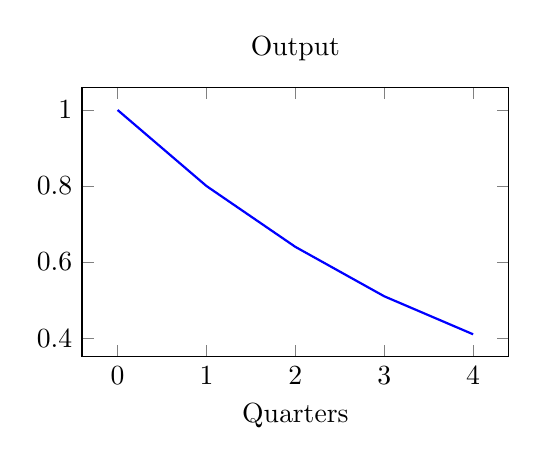
\begin{tikzpicture}\begin{axis}[width=7cm,height=5cm,xlabel={Quarters},title={Output}]
\addplot[blue,thick] coordinates {(0,1)(1,0.8)(2,0.64)(3,0.51)(4,0.41)};
\end{axis}\end{tikzpicture}\caption{IRF}\end{figure}
\bibliographystyle{aer}
\bibliography{refs}
\end{document}
